% Latex template: mahmoud.s.fahmy@students.kasralainy.edu.eg
% For more details: https://www.sharelatex.com/learn/Beamer

\documentclass{beamer}					  % Document class

\usepackage[portuguese]{babel}			  % Set language
\usepackage[utf8x]{inputenc}			  % Set encoding

\mode<presentation> {					  % Set options
  \usetheme{default}					    % Set theme
  \usecolortheme{default} 				% Set colors
  \usefonttheme{default}  				% Set font theme
  \setbeamertemplate{caption}[numbered]	% Set caption to be numbered
}

\setbeamertemplate{navigation symbols}{}
\setbeamertemplate{footline}[frame number]
\setbeamercovered{transparent}

% Uncomment this to have the outline at the beginning of each section highlighted.
%\AtBeginSection[]
%{
%  \begin{frame}{Outline}
%    \tableofcontents[currentsection]
%  \end{frame}
%}

\usepackage{graphicx}					% For including figures
\usepackage{booktabs}					% For table rules
\usepackage{hyperref}					% For cross-referencing
\usepackage{caption}                    % Allows more control over captions in figs and tables

\title{Revisão de Atividades da FAC}	% Presentation title
%\author{Author One}					% Presentation author
\institute{LNLS.DAC.FAC}				% Author affiliation
\date{2023-10-27 -- 2023-11-17}			% Today's date	


\begin{document}



\begin{frame}
  \titlepage
  \href{https://github.com/lnls-fac/doc-review-dac-fac}{\beamergotobutton{Link para o repo github desta apresentação: https://github.com/lnls-fac/doc-review-dac-fac}}
  \href{https://www.overleaf.com/read/sbdjxtzfchrm}{\beamergotobutton{Link para o projeto overleaf destas notas}}
\end{frame}

\begin{frame}{Outline}
  \tableofcontents
\end{frame}


\section{Recuperação de Máquina - 10-16/11}

\begin{frame}{10-13/11 Recuperação de Máquina}
    \begin{minipage}{0.4\textwidth}
        \scriptsize{
        \begin{itemize}
    		\item 10/11 (sexta) - subsistemas ligados, sem FOFB. Injeção de 100 mA, BBA em baixa corrente.
            \item 11/11 (sábado) - algumas queda de feixe por RF na madrugada, falha Regatron de sextupolos do SI.
            \item 13/11 (segunda) - órbita de referência, medida matriz resposta (já usamos a matriz AC), análise LOCO, correção de ótica e acoplamento, equalização dos BPMs.
        \end{itemize}}
    \end{minipage}
    \begin{minipage}{0.58\textwidth}
        \captionsetup[figure]{font=tiny}
        \begin{figure}[H]
        	\centering
            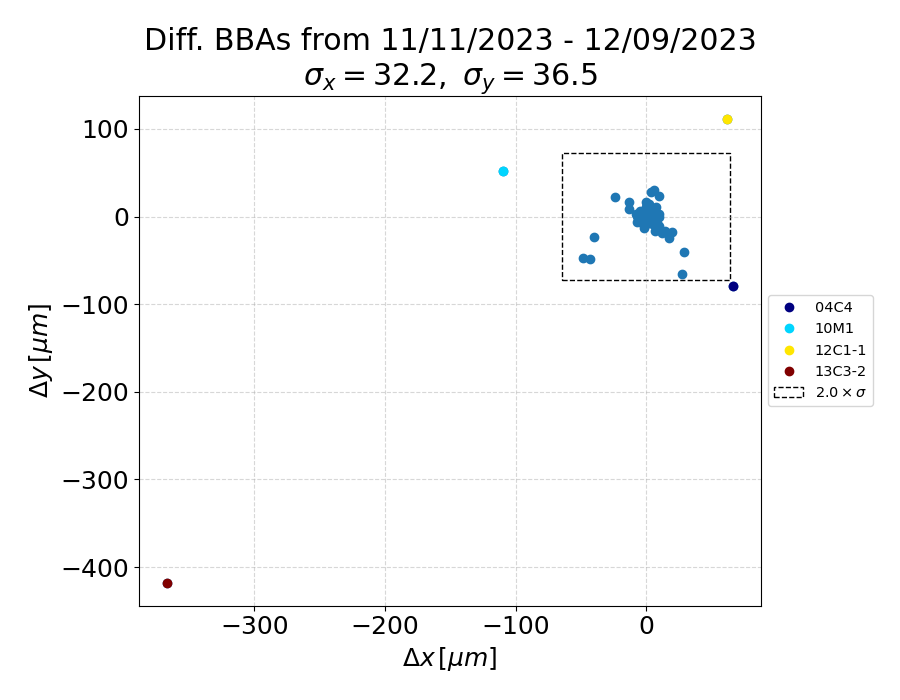
\includegraphics[width=1\textwidth]{2023-11-17/figures/diff_to_bba_after_september23_shutdown.png}
            \caption{\tiny{Diferença entres BBAs: novembro em relação ao de setembro. Variações grandes provavelmente devido a retirada de placas de BPMs durante a parada (informada previamente à recuperação pelo Augusto).}}
            \label{fig:bba}
        \end{figure}
    \end{minipage}
\end{frame}
\begin{frame}{14-16/11 Recuperação de Máquina}
    \begin{minipage}{0.45\textwidth}
        \begin{itemize}
        \scriptsize{
            \item 14/11 (terça) 
            \begin{itemize}
            \scriptsize{
                \item interlock ``sobre-corrente na carga'' em corretoras lentas (CH e CV) do mesmo bastidor 20C1 e 20C4. Troca do bastidor parece ter resolvido. 
                \item tentativa de ajuste de LLRF para evitar instabilidade de feixe. Identificação de arco nos guias da SSA3;}
            \end{itemize}
            \item 15/11 (quarta) - conserto do SSA3 e recuperação de máquina. Feixe liberado para usuários às 20h.
            \item 16/11 (quinta) - testes de vácuo na SABIÁ com campo do DELTA52 limitado a fase de 9 mm (Potência do EPU)}
    	\end{itemize}
    \end{minipage}
    \begin{minipage}{0.53\textwidth}
        \captionsetup[figure]{font=tiny}
        \begin{figure}[H]
        	\centering
            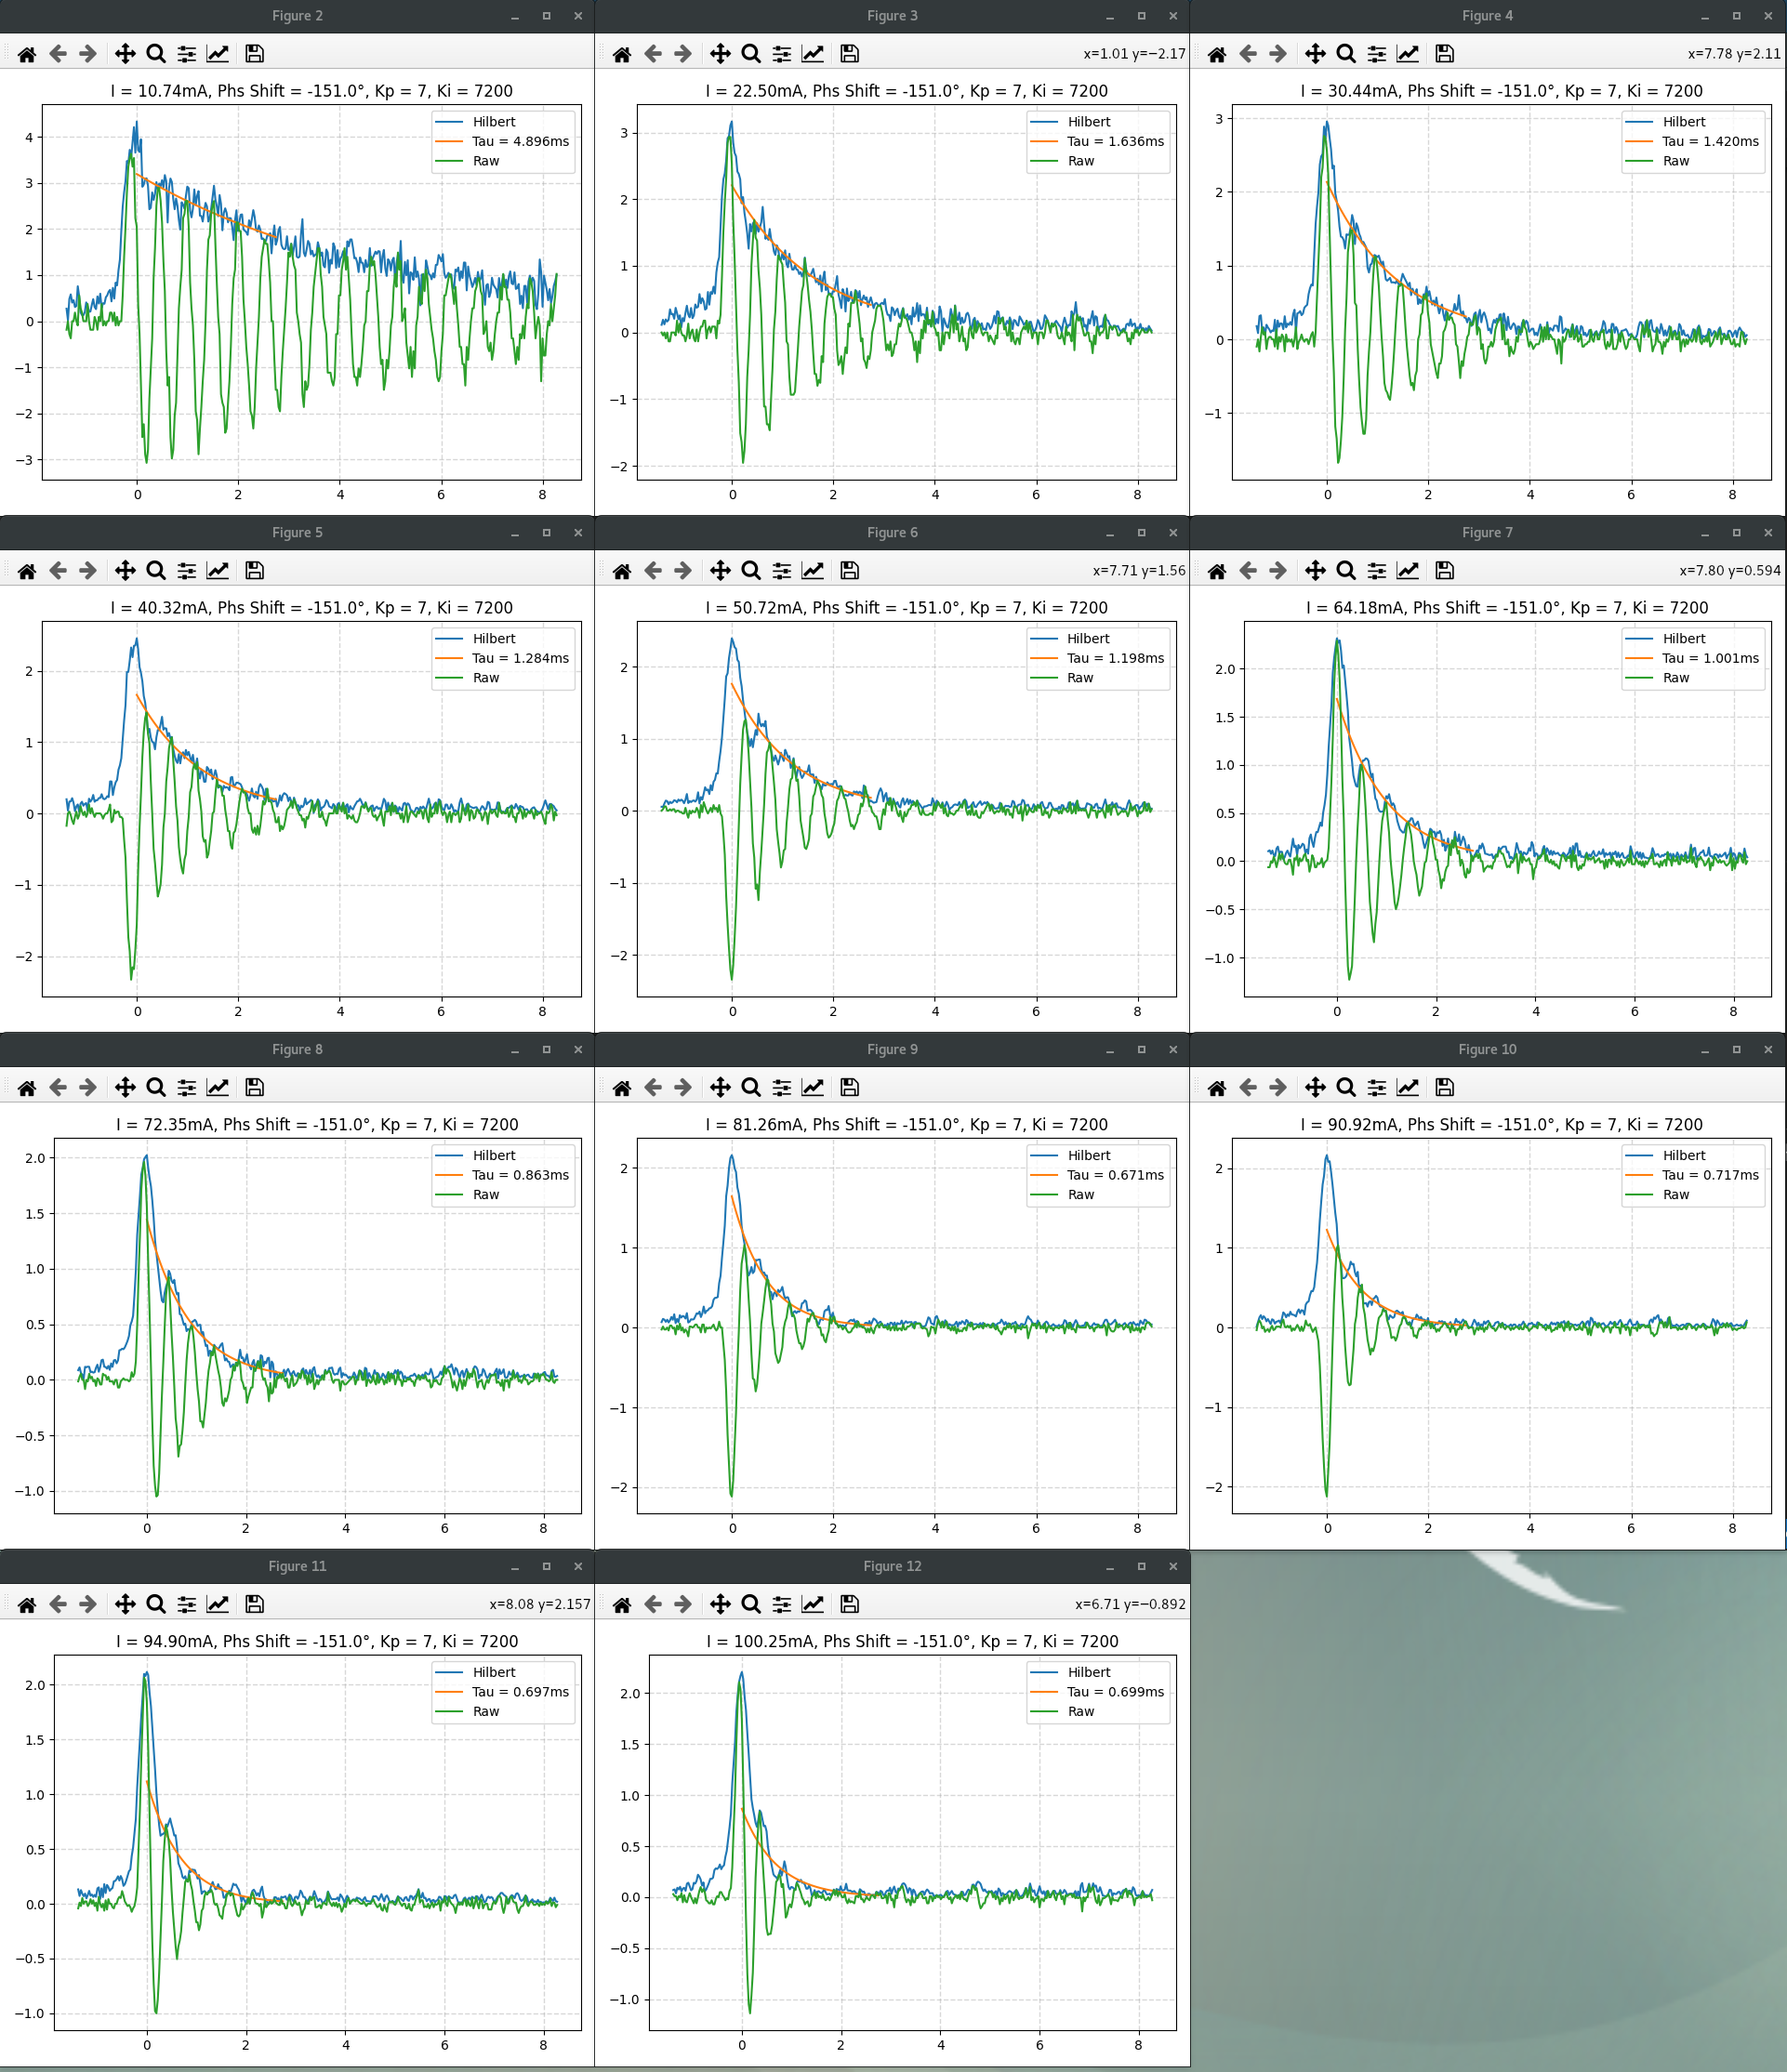
\includegraphics[width=\textwidth]{2023-11-17/figures/beam_damping_times_vs_current.png}
            \caption{\tiny{Damping times of mode-0 vs stored current in uniform filling.}}
            \label{fig:llrf_damping1}
        \end{figure}
    \end{minipage}
\end{frame}

\begin{frame}{Perturbação NLK}
\begin{itemize}
\small{
    \item NLK foi realinhado durante a parada para posição em que perturbação do pulso principal deveria ser nula. Agora as bobinas de compensação deveriam combater apenas campos de eddy currents
    \item Não tivemos tempo para encontrar novos valores de amplitude e delay das bobinas de compensação, atualmente estamos com a config. anterior e a injeção não está transparente. 
    \item Tabela feedforward DELTA e injeção transparente são prioridades para o estudo da próxima semana. 
    }
\end{itemize}
    \begin{figure}[H]
        	\centering
            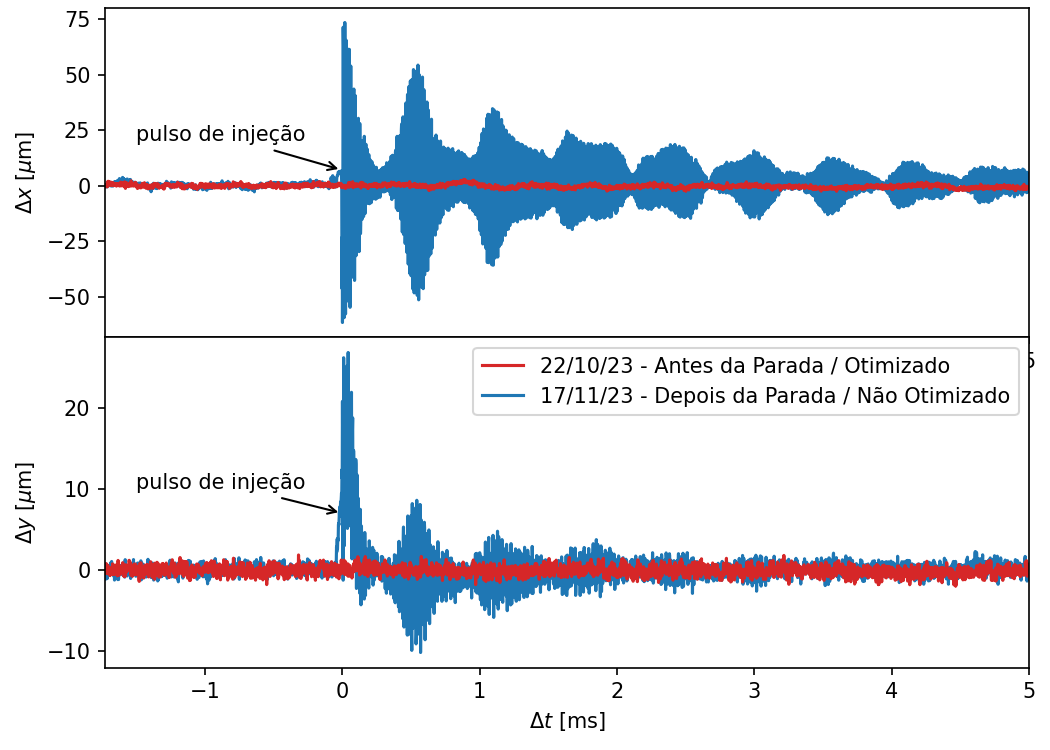
\includegraphics[width=0.6\textwidth]{2023-11-17/figures/injection_perturbation_after_november23_shutdown.png}
            % \caption{Perturbação do NLK durante a injeção, antes (vermelho) e depois (azul) da parada.}
            \label{fig:llrf_damping2}
        \end{figure}
\end{frame}

\section{Atividades - DELTA52}

\begin{frame}{DELTA52 - Medidas Oficiais}
    \begin{itemize}
            \item Medidas de mapas com sensor Hall e integrais de campo com fio esticado no plano e fora do plano.
    \end{itemize}
    \begin{figure}[H]
    		\centering
            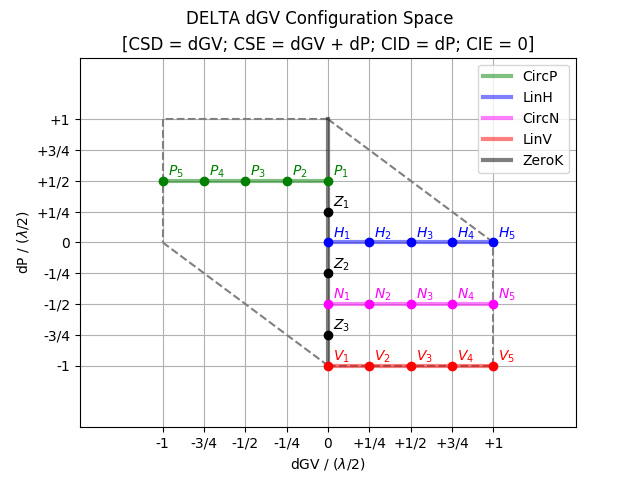
\includegraphics[width=.8\textwidth]{2023-11-17/figures/id-delta-dgv-config-space.png}
            \caption{Configurações mapeadas com sensor Hall.}
            \label{fig:delta-config-space}
    \end{figure}
\end{frame}

\begin{frame}{DELTA52 - Medidas Oficiais}
    \begin{itemize}
            \item Medidas de mapas com sensor Hall e integrais de campo com fio esticado no plano e fora do plano.
    \end{itemize}
    \begin{figure}[H]
    		\centering
            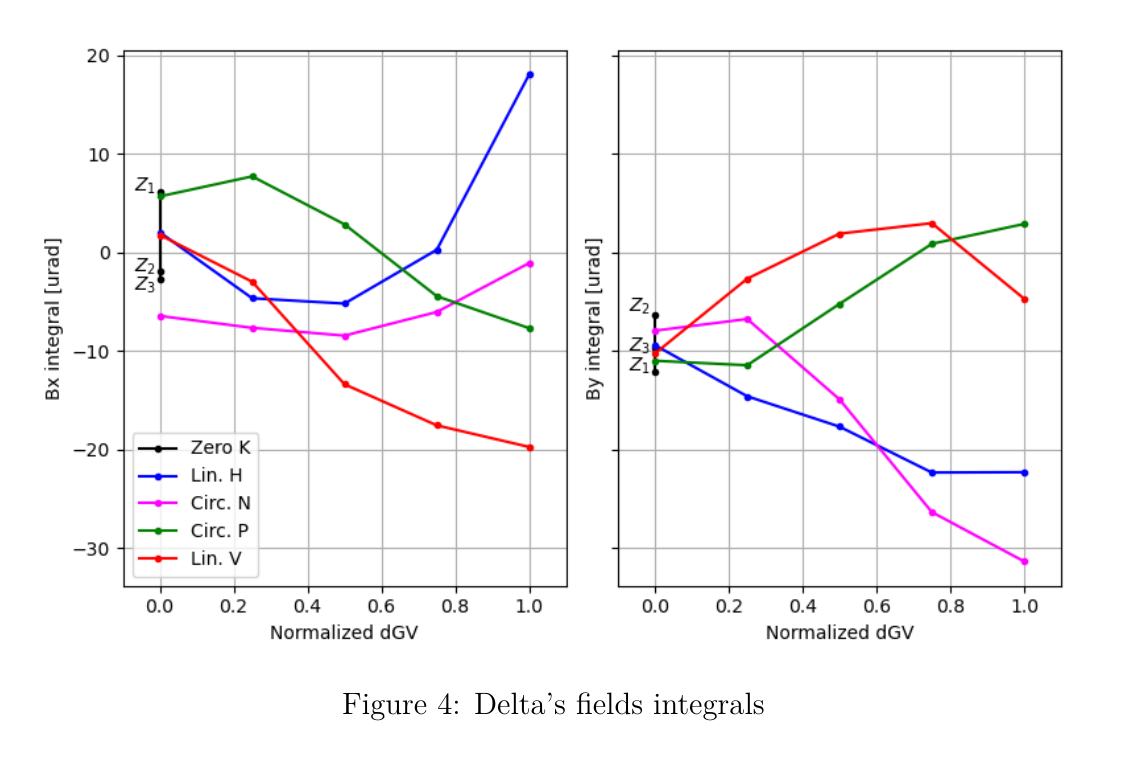
\includegraphics[width=.8\textwidth]{2023-11-17/figures/delta52-fields.png}
            \caption{Configurações mapeadas com sensor Hall.}
            \label{fig:delta-int}
    \end{figure}
\end{frame}

\begin{frame}{DELTA52 - Análise de AD \href{https://cnpemcamp.sharepoint.com/:b:/s/FAC/EaZonslbB0pBja96L0moRwMBH7-Uh5Bat4ToycITMlczMA?e=2btWUd}{\beamergotobutton{Link para relatório}}}
    \begin{itemize}
            \item AD calculada com mapa de kick em y=0 (mapa de campo) e estendido.
            \item Artefato de correção de cross-talk Bx/Bz sensor Hall
    \end{itemize}
    \begin{figure}[H]
    		\centering
            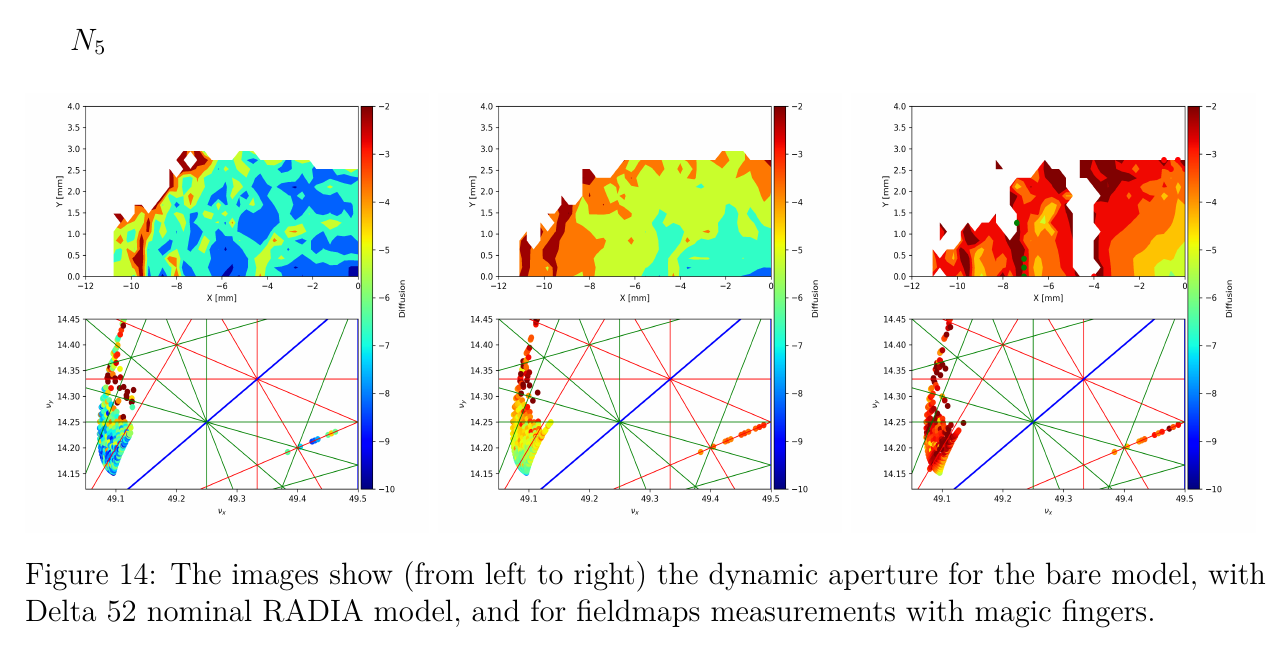
\includegraphics[width=.9\textwidth]{2023-11-17/figures/ad-n5.png}
            \label{fig:dynapt1}
    \end{figure}
\end{frame}

\begin{frame}{DELTA52 - Análise de AD \href{https://cnpemcamp.sharepoint.com/:b:/s/FAC/EaZonslbB0pBja96L0moRwMBH7-Uh5Bat4ToycITMlczMA?e=2btWUd}{\beamergotobutton{Link para relatório}}}
    \begin{itemize}
            \item AD calculada do N5 com mapa de kick a partir das integrais de fio esticado.
    \end{itemize}
    \begin{figure}[H]
    		\centering
            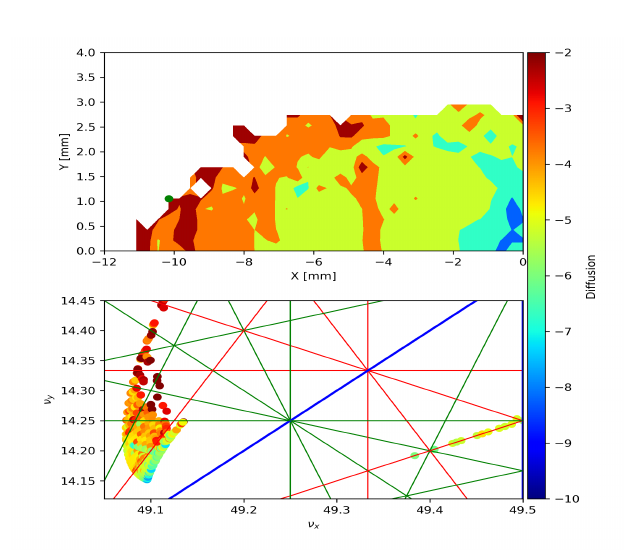
\includegraphics[width=.6\textwidth]{2023-11-17/figures/ad-n5-swire.png}
            \label{fig:dynapt2}
    \end{figure}
    \begin{itemize}
            \item Pessoal do IMA analisando os motivos deste artefato introduzido na correção do crosstalk.
    \end{itemize}
\end{frame}

\begin{frame}{DELTA52 - Teste com campo/polarização}
    \begin{itemize}
            \item Limitado dGV (CSD) em 9mm : potência menor que do EPU em campo máximo.
            \item Aumento gradativo de campo/potência, passos de 5\%.
            \item LinH : 95\%, LinV : 85\%, CircN : 55\%, CircP : 45\%
            \item Não houve nenhuma alteração significativa de pressão no FE do anel e nem na SABIÁ (Gustavo acompanhou).
    \end{itemize}
\end{frame}

\begin{frame}{DELTA52 - Teste com campo/polarização}
    \begin{itemize}
            \item Efeitos desprezíveis nos tamanhos, ângulo, e eficiência de injeção.
            \begin{figure}[H]
    		\centering
            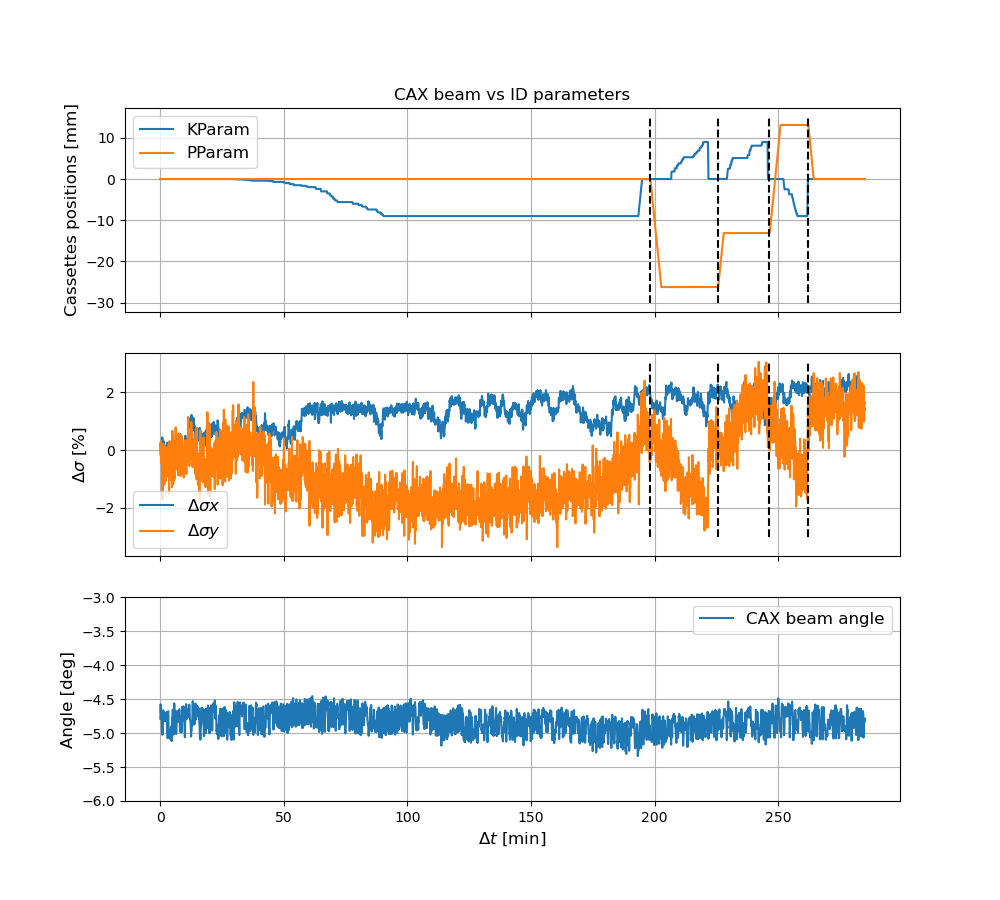
\includegraphics[width=.7\textwidth]{2023-11-17/figures/CAX_beam_id_param.png}
            \caption{Efeitos do DELTA no feixe observado na Carcará.}
            \label{fig:cax_param}
    \end{figure}
    \end{itemize}
\end{frame}

\begin{frame}{DELTA52 - Teste com campo/polarização}
            \begin{figure}[H]
    		\centering
            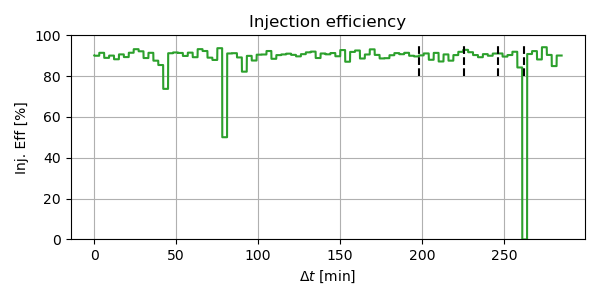
\includegraphics[width=1\textwidth]{2023-11-17/figures/inj_eff.png}
            \caption{Efeitos do DELTA na eficiência de injeção.}
            \label{fig:inj_eff}
    \end{figure}
\end{frame}

\begin{frame}{DELTA52 - Teste com campo/polarização}
            \begin{figure}[H]
    		\centering
            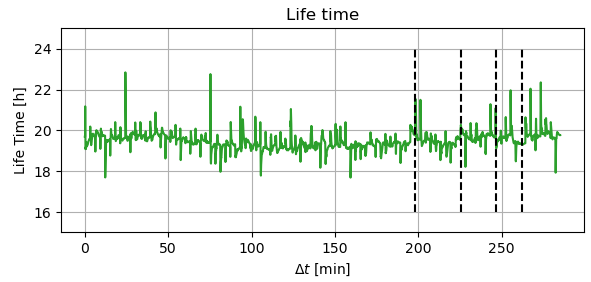
\includegraphics[width=1\textwidth]{2023-11-17/figures/lifetime.png}
            \caption{Efeitos do DELTA no tempo de vida.}
            \label{fig:lifetime}
    \end{figure}
\end{frame}

\begin{frame}{DELTA52 - Teste com campo/polarização}
    \begin{itemize}
            \item Desvio de sintonia pequeno durante mudança de polarização, compatível com valores esperados.
            \begin{figure}[H]
    		\centering
            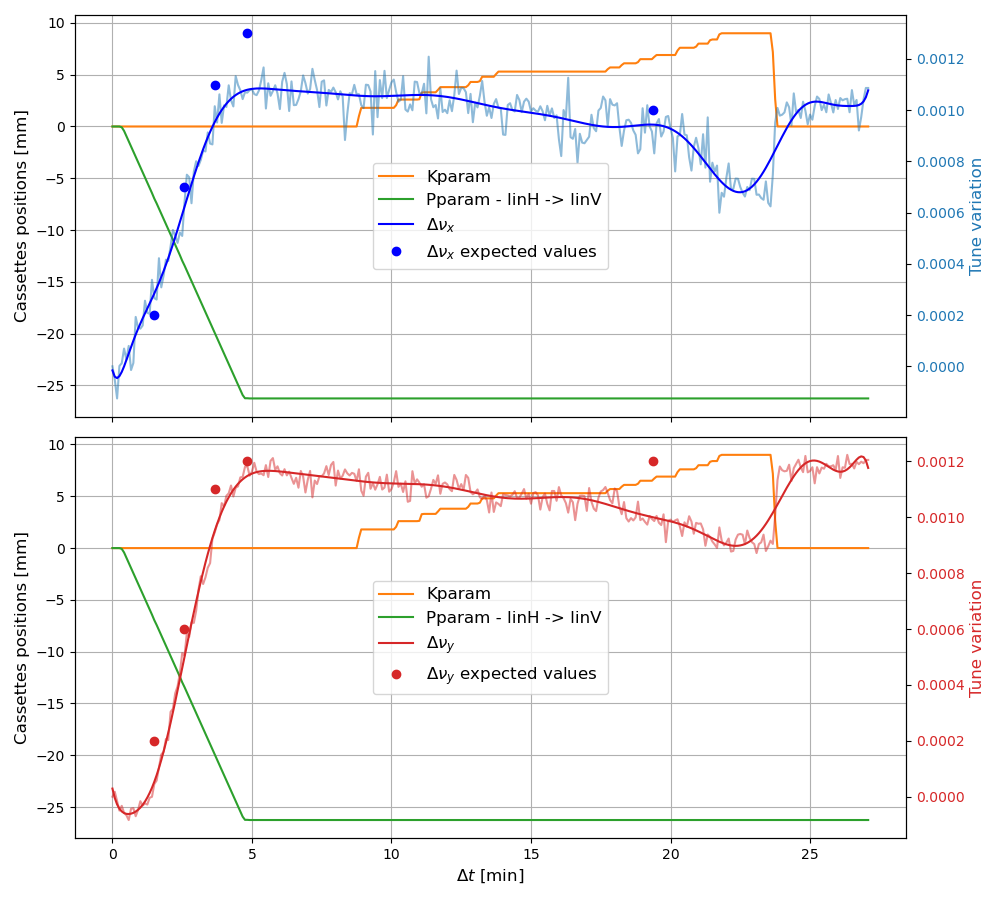
\includegraphics[width=.7\textwidth]{2023-11-17/figures/tune_linh_linv.png}
            \caption{Efeitos do DELTA na ótica linear}
            \label{fig:linh_linv}
        \end{figure}
    \end{itemize}
\end{frame}


\section{Atividades - Janela de equalização dos BPMs}

\begin{frame}{Janela de equalização do BPMs}
    \begin{itemize}
        \scriptsize
        \item Antes a equalização era feita por um script que nem sempre funcionava devido ao desalinhamento temporal das aquisições trigadas. A compensação do impacto na órbita também não era feito de maneira sistemática (diferenças de órbitas).
        \item Agora, criamos um método de identificação dos semiciclos: a equalização sempre funciona. A compensação do impacto na órbita é calculada exatamente a partir dos dados das antenas.
    \end{itemize}
    \begin{figure}[H]
   		\centering
        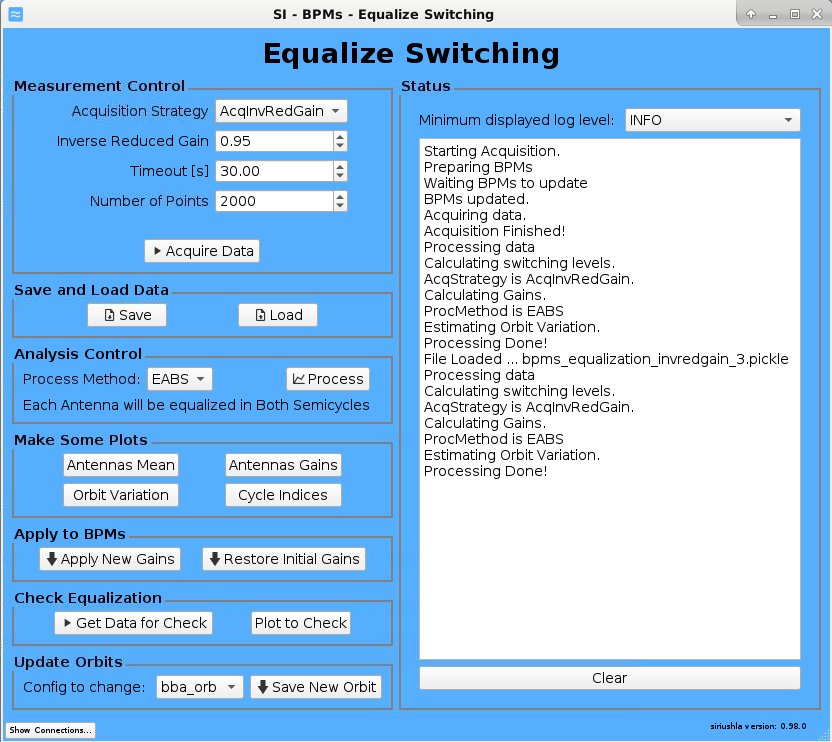
\includegraphics[width=.48\textwidth]{
            2023-11-17/figures/bpms_equalization_window.png}
        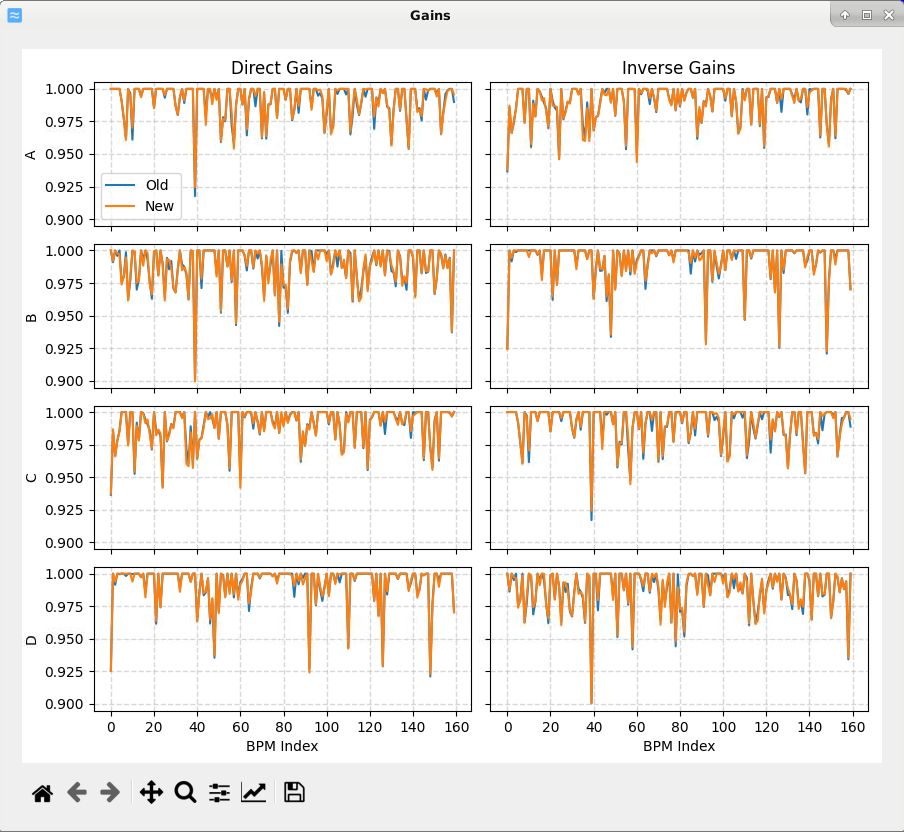
\includegraphics[width=.48\textwidth]{2023-11-17/figures/bpms_gains.png}
        \label{fig:bpmseq_window}
    \end{figure}
\end{frame}

\section{References}


\end{document}
